\chapter{Quantifying Characteristics of the FD PMT}\label{Ch:PMTCharacter}

Characterising the PMT at 600V and 900V
\begin{itemize}
\item Using the characteristics of the PMT at 900V as a baseline
\item Measure linearity
\item ND filters vs Two LED method
\item Pulse shape?
\item temperature effects
\item dark noise?
\end{itemize}

\begin{figure}
\centering
\includegraphics[width=\textwidth]{chapters/graphs/PMTchar/pmt_linearity_100V_privitera.png}
\caption{Previous PMT linearity test done by Privitera et. al. 1999 with Neutral density filters.}
\end{figure}

\begin{figure}
\centering
\begin{subfigure}[b]{\textwidth}
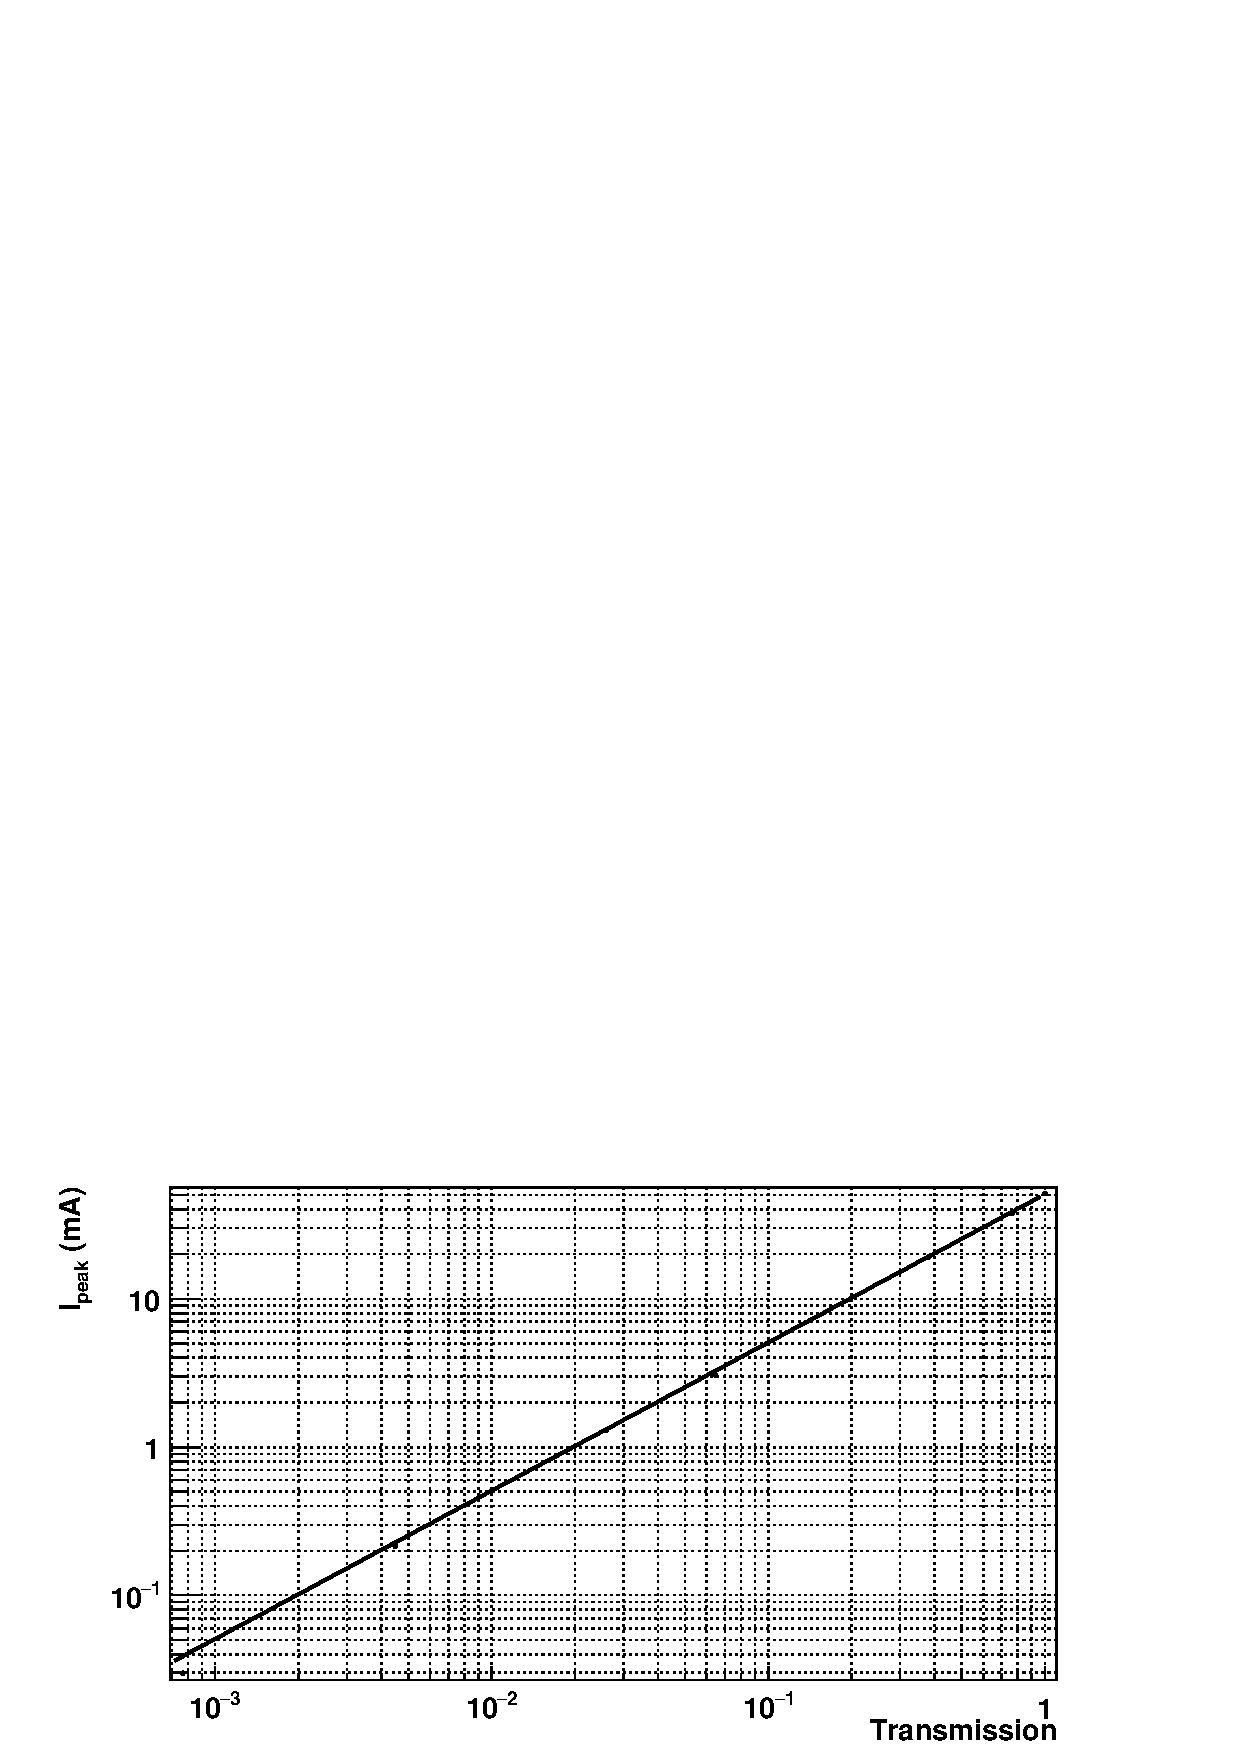
\includegraphics[width=\textwidth]{chapters/graphs/PMTchar/PMT900V_linearityNDmethod.pdf}
\caption{•}
\end{subfigure}
\begin{subfigure}[b]{\textwidth}
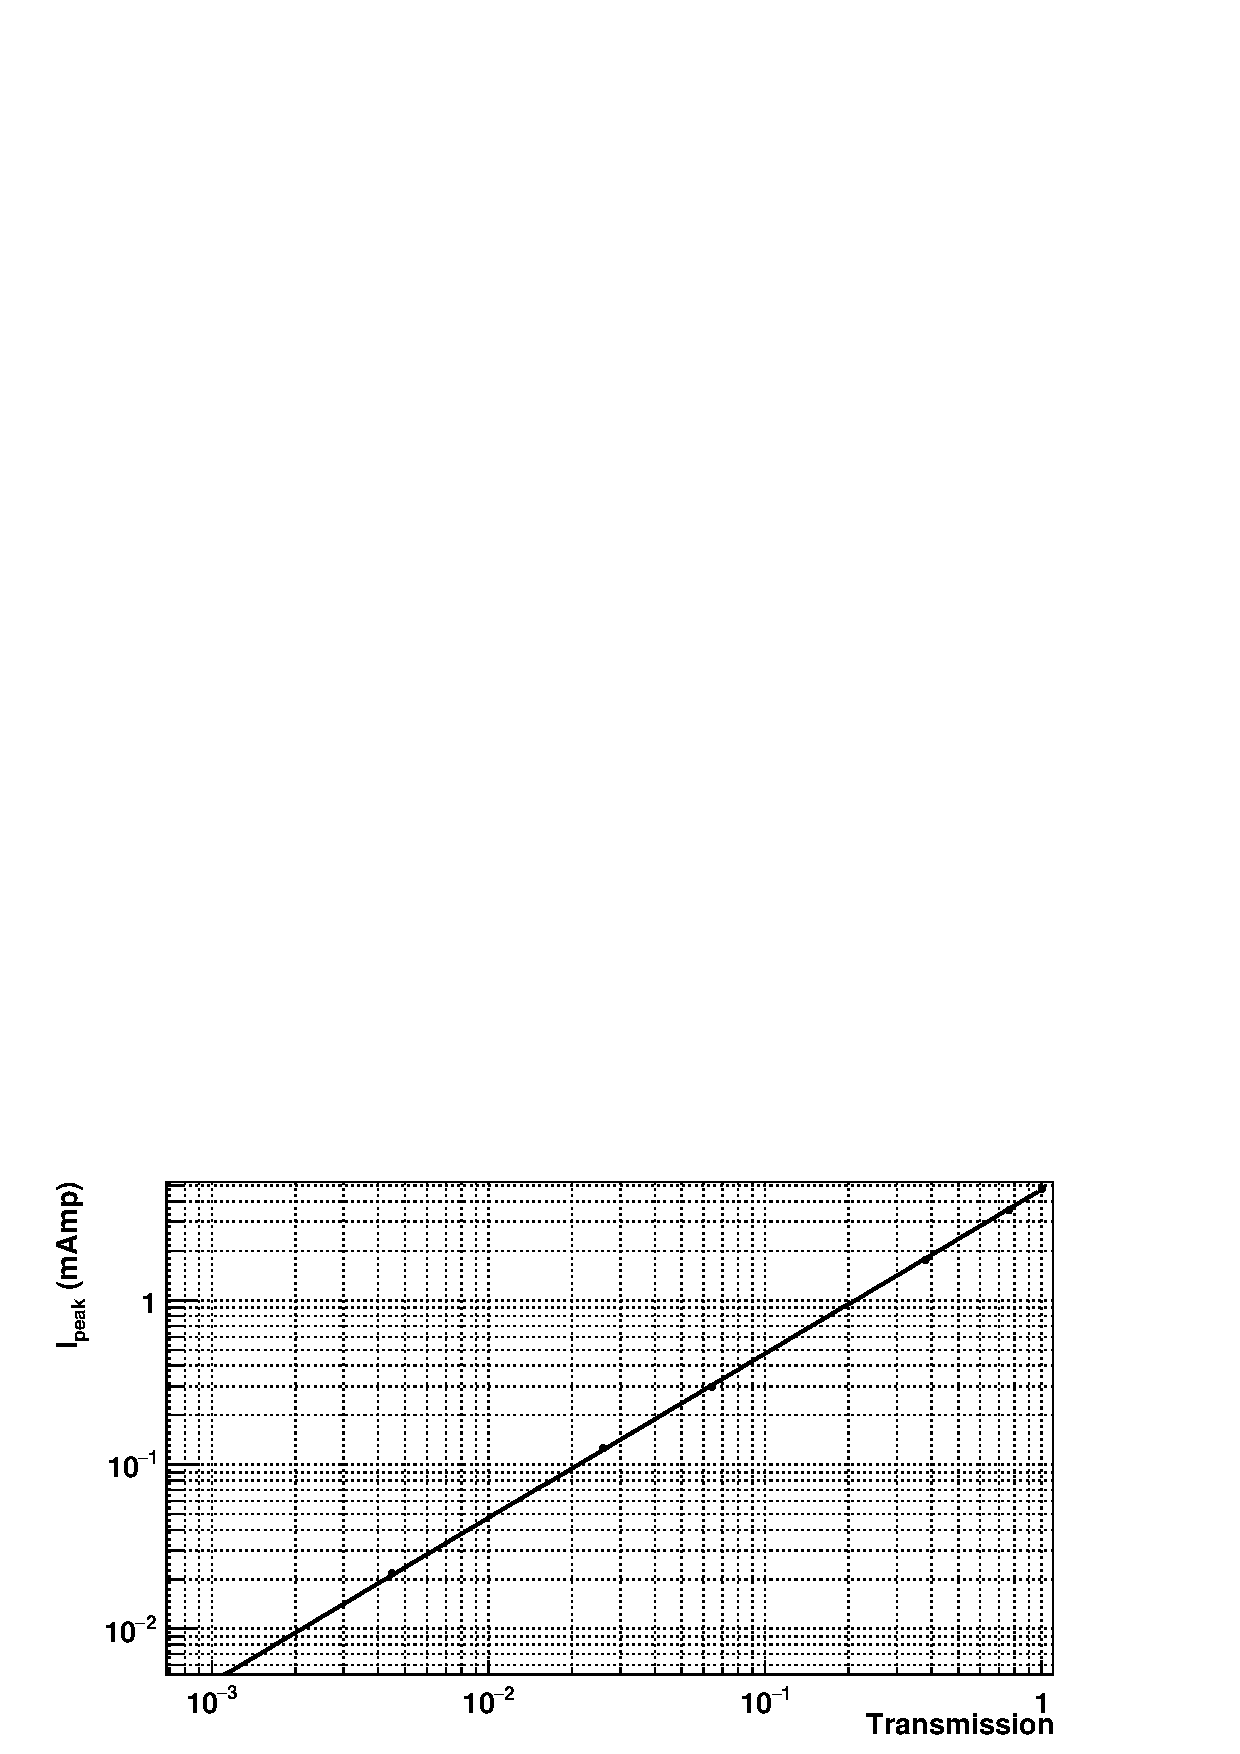
\includegraphics[width=\textwidth]{chapters/graphs/PMTchar/PMT600V_linearityNDmethod.pdf}
\caption{•}
\end{subfigure}
\caption{Neutral density method at 900V and 600V.}
\end{figure}

\begin{figure}
\centering
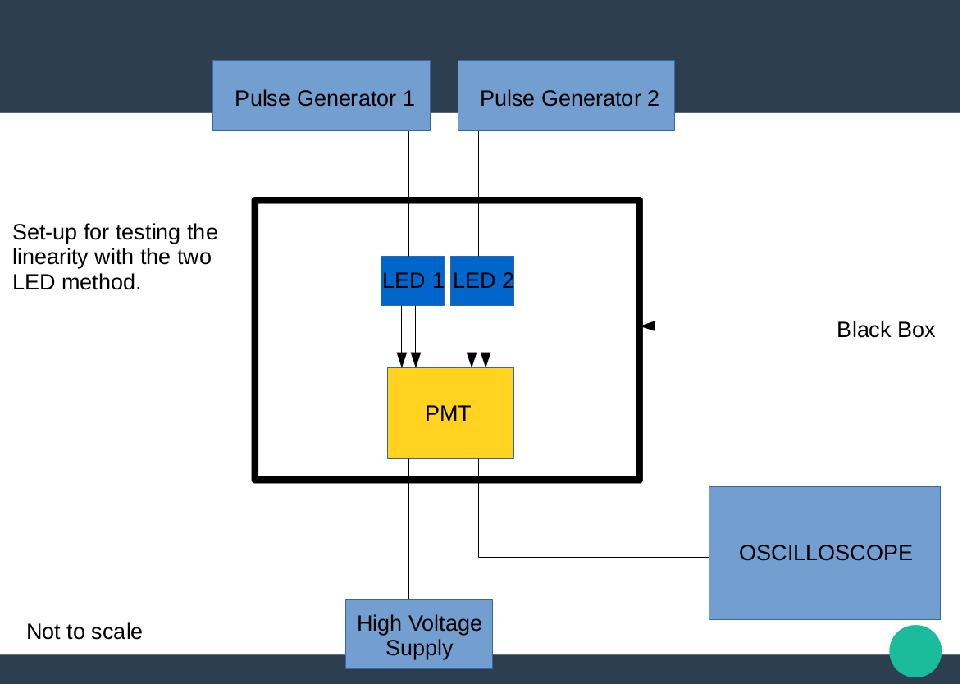
\includegraphics[width=\textwidth]{chapters/graphs/PMTchar/diagram_TwoLEDmethod.pdf}
\end{figure}

\begin{figure}
\centering
\begin{subfigure}[b]{\textwidth}
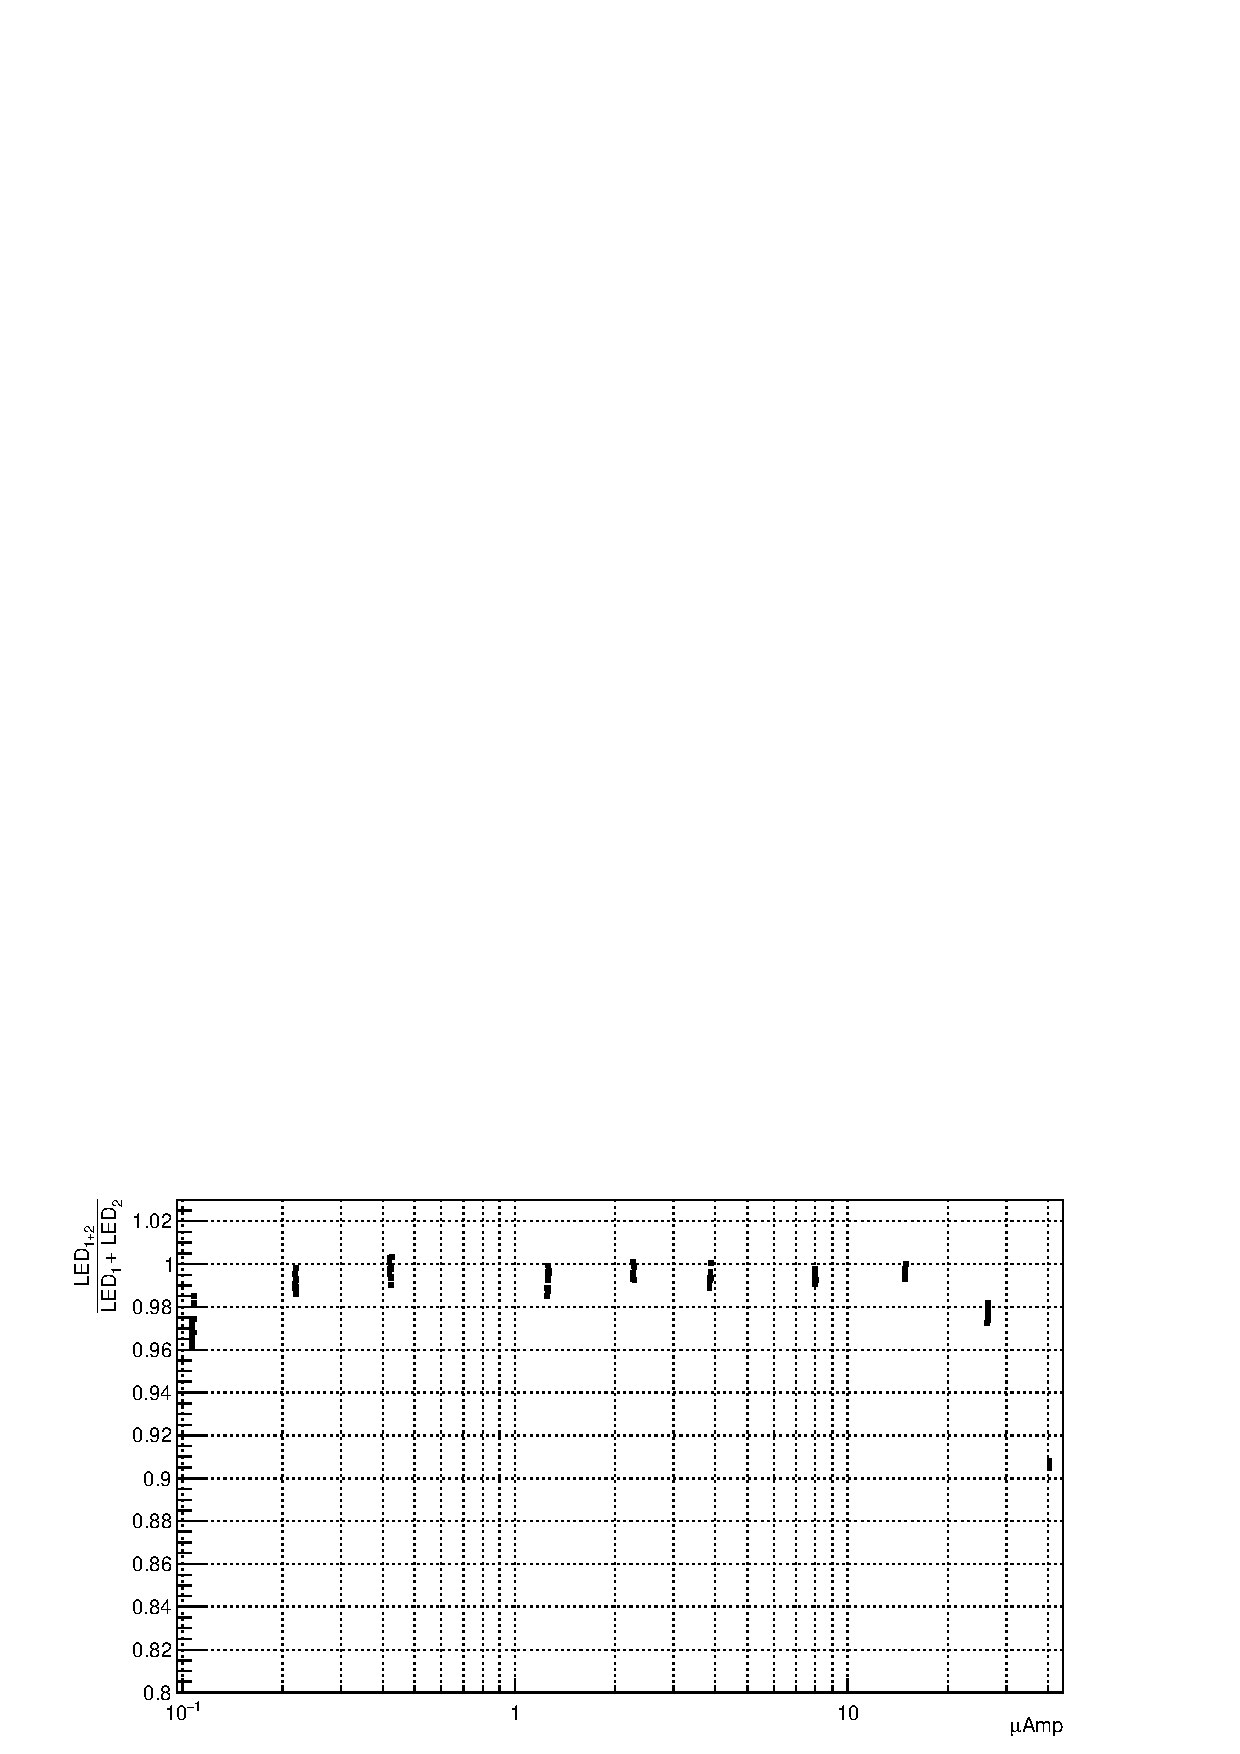
\includegraphics[width=\textwidth]{chapters/graphs/PMTchar/PMT900V_linearity2LEDmethod.pdf}
\caption{•}
\end{subfigure}
\begin{subfigure}[b]{\textwidth}
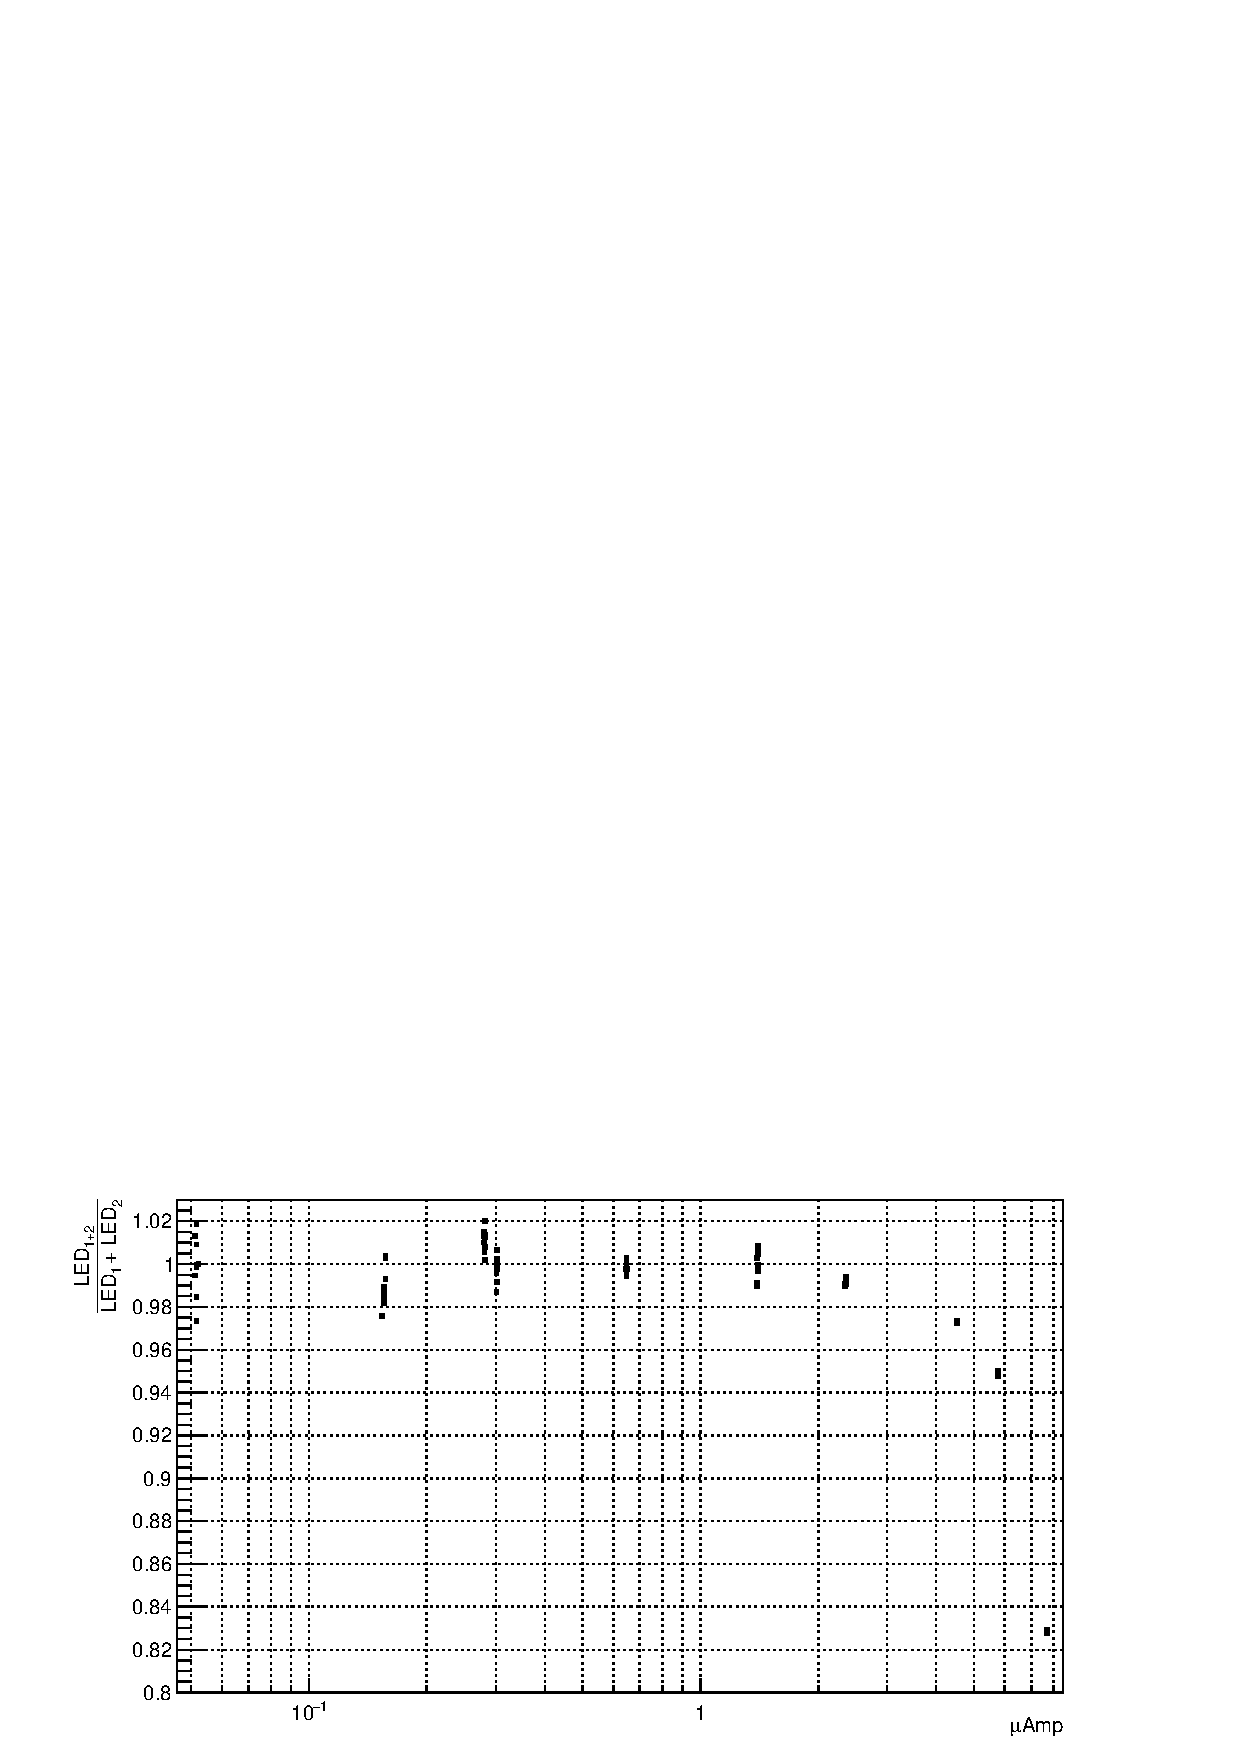
\includegraphics[width=\textwidth]{chapters/graphs/PMTchar/PMT600V_linearity2LEDmethod.pdf}
\caption{•}
\end{subfigure}
\caption{Two LED method at 900V and 600V.}
\end{figure}